\section*{Annexes}
\subsection*{Annexe 1 -- Aide au calcul}
\begin{center}
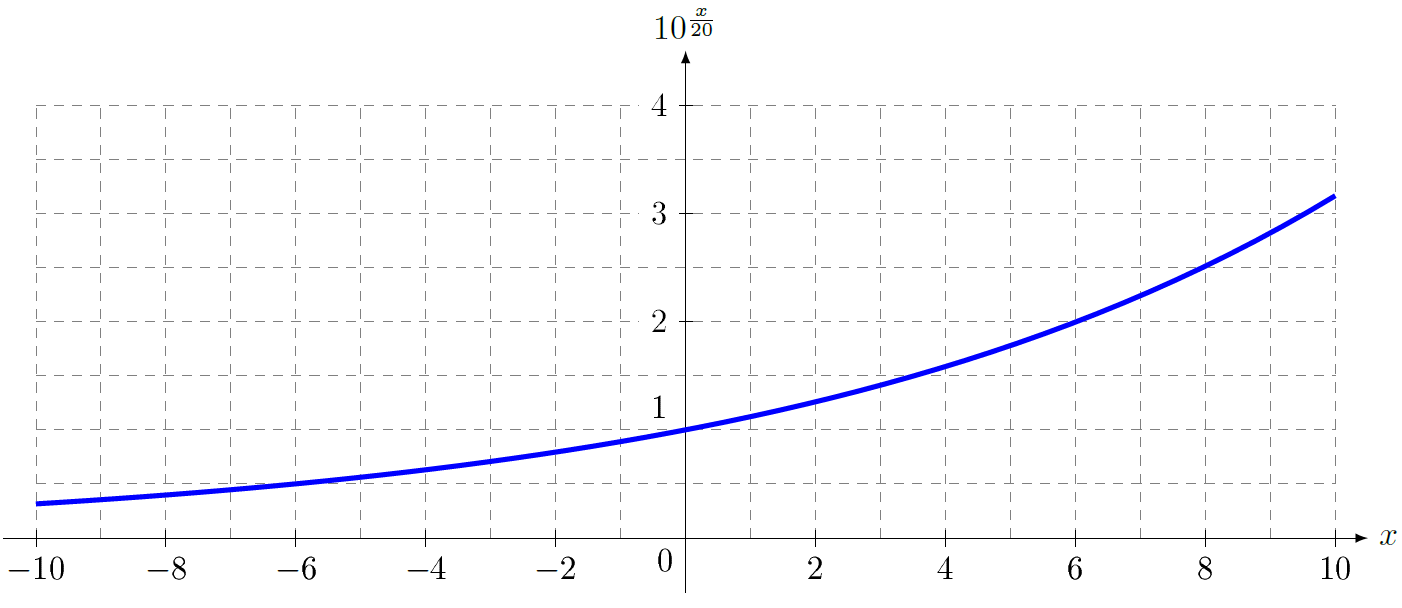
\includegraphics[width=.8\linewidth]{ann_01}

\textit{Fonction $f(x)=10^{\dfrac{x}{20}}$}
\end{center}

\subsection*{Annexe 2 -- Analyse fonctionnelle}
\begin{multicols}{2}
\begin{center}
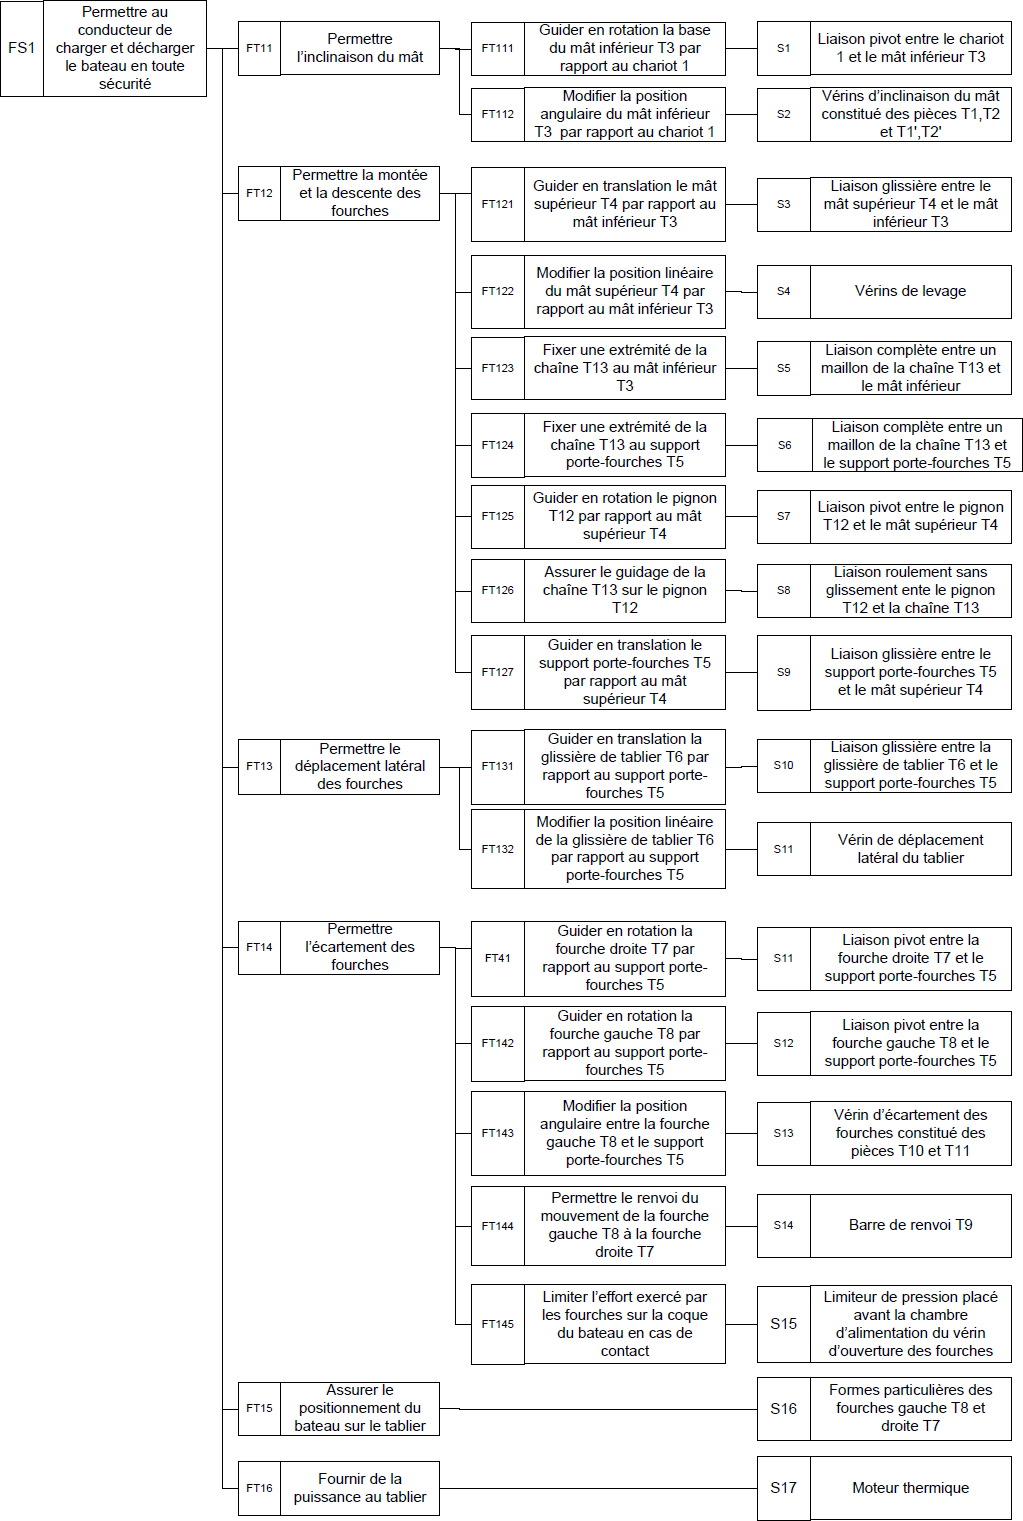
\includegraphics[height=4cm]{ann_02}

\textit{Diagramme de cas d'utilisation}
\end{center}

\begin{center}
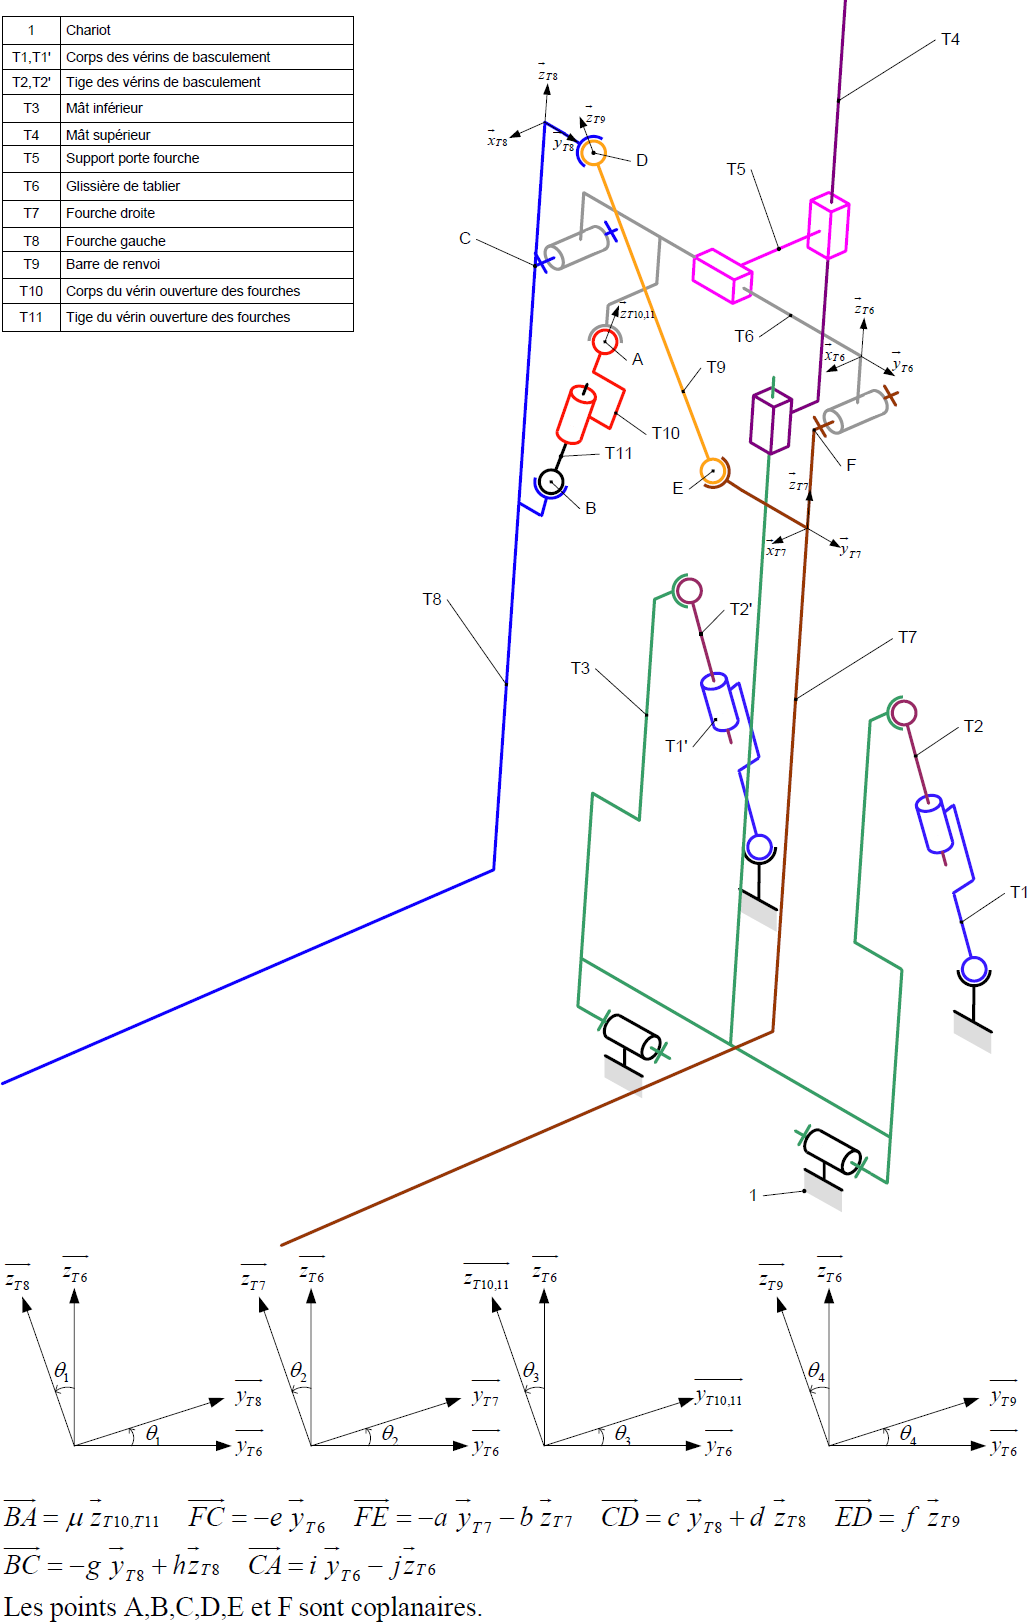
\includegraphics[height=4cm]{ann_03}

\textit{Diagramme de contexte}
\end{center}
\end{multicols}
\subsection*{Annexe 3 -- Vues du bassin}
\begin{center}
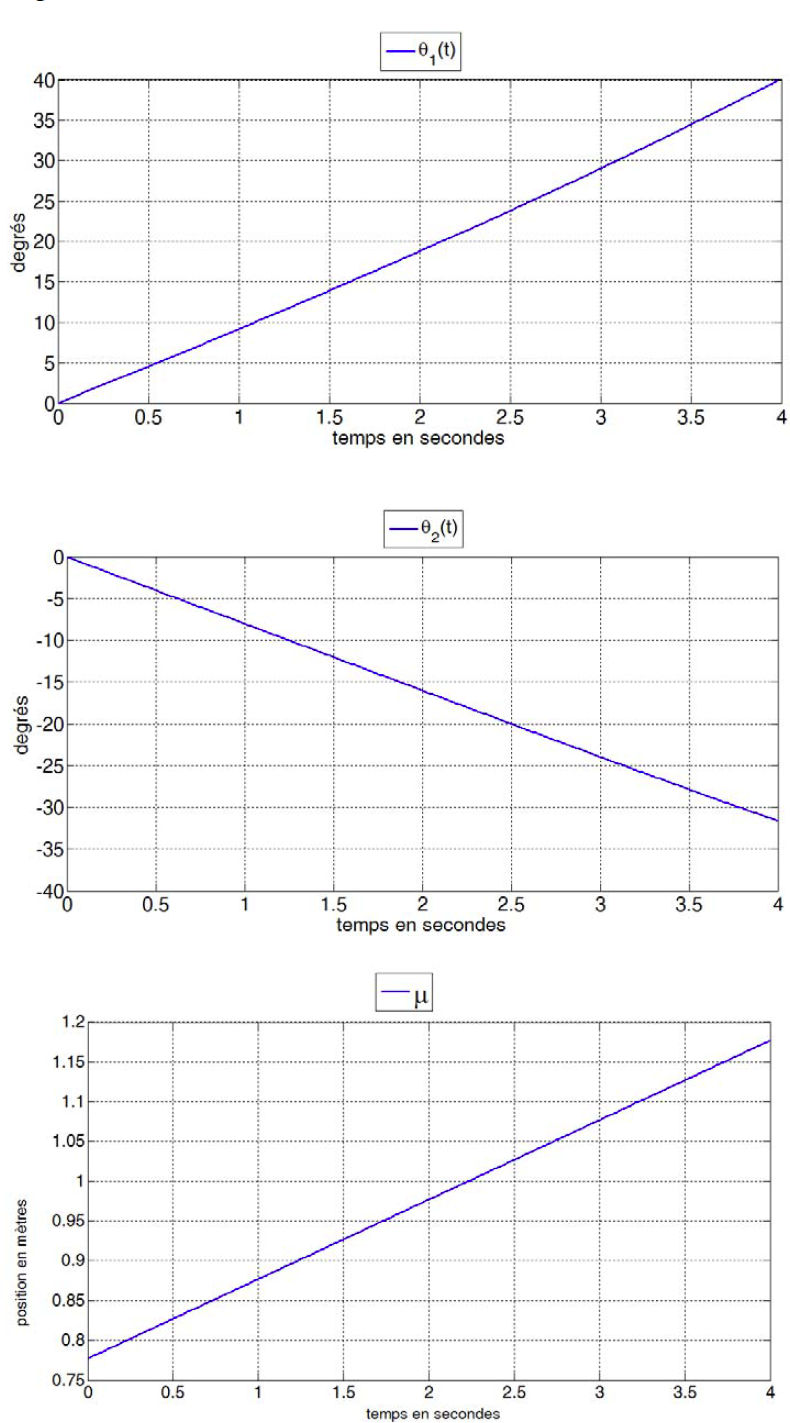
\includegraphics[width=\linewidth]{ann_04}

\textit{Dimensions : \SI{140}{m} de long x \SI{5}{m} de largeur x \SI{3}{m} de profondeur }
\end{center}

\subsection*{Annexe 4 -- Exrtrait du receuil des exigences}
\begin{center}
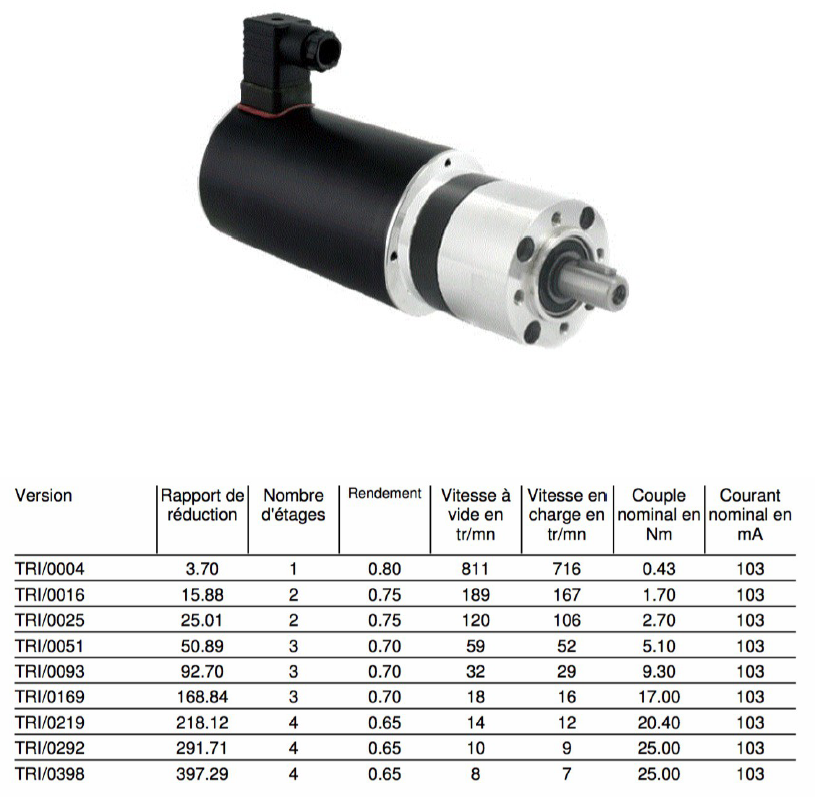
\includegraphics[width=\linewidth]{ann_05}

\textit{Diagramme des exigences (partiel) }
\end{center}
\begin{center}
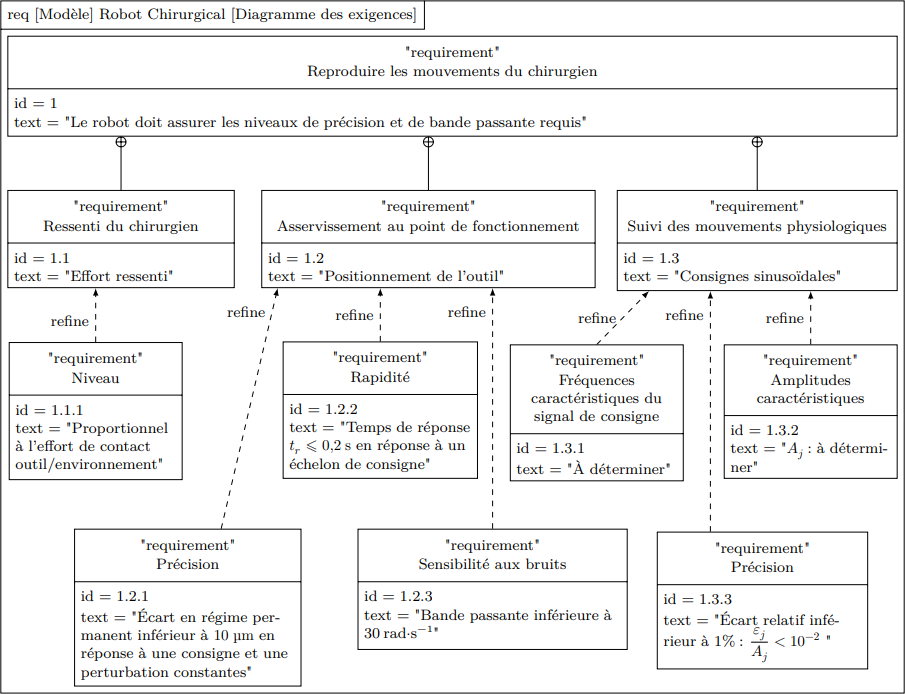
\includegraphics[width=\linewidth]{req}

\textit{Tableau des exigences (partiel)}
\end{center}


\subsection*{Annexe 5 -- Architecture organique du système}
Le bassin de traction est composé d'un bassin rempli d'eau, d'un batteur générant une houle, de deux rails 
sur lesquels un chariot est mis en mouvement pour générer une vitesse relative d'une maquette par 
rapport à la surface de l'eau. 

\begin{center}
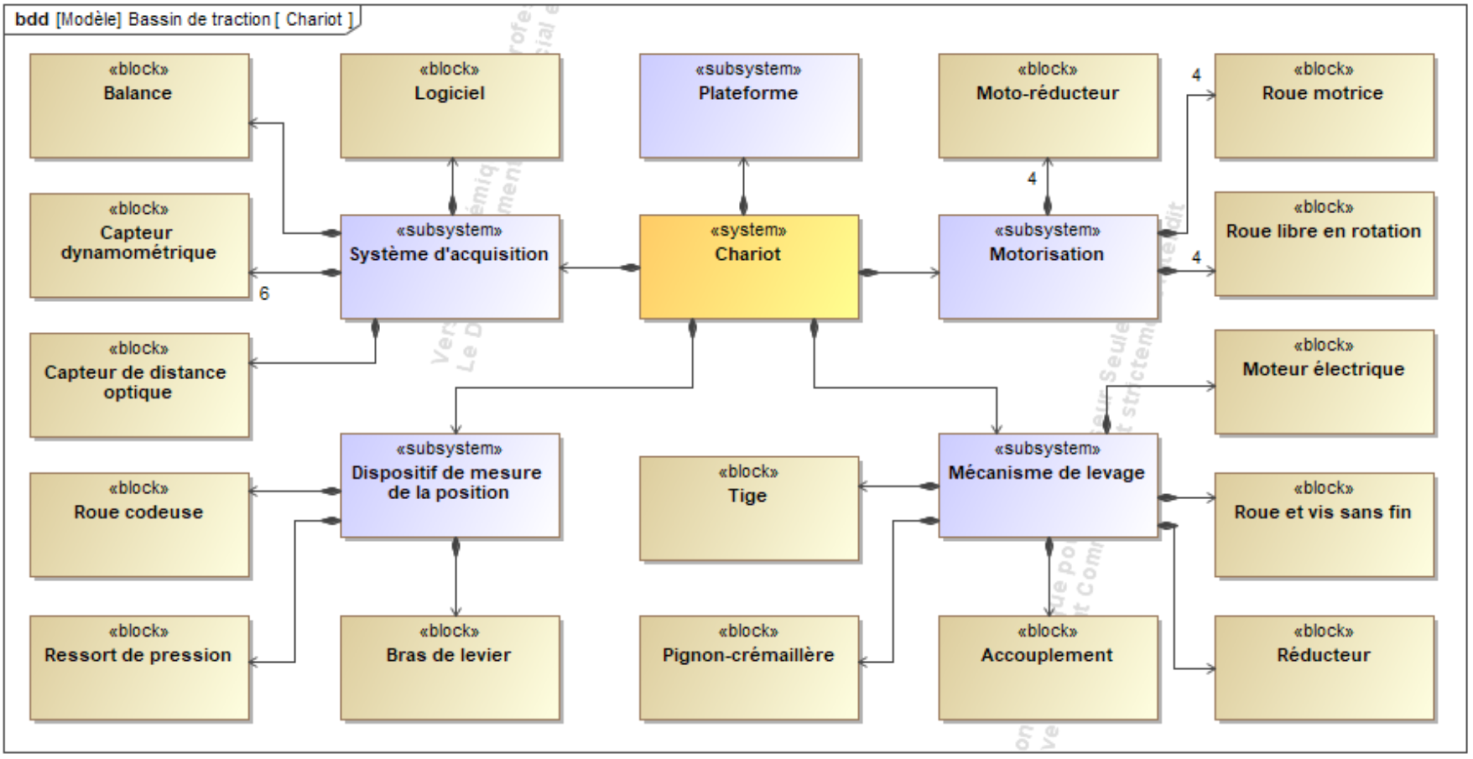
\includegraphics[width=\linewidth]{ann_06}

\textit{Diagramme de Définition de Blocs du Bassin de Traction }
\end{center}

\subsection*{Annexe 6 -- Modélisation du chariot et de son guidage}
\begin{center}
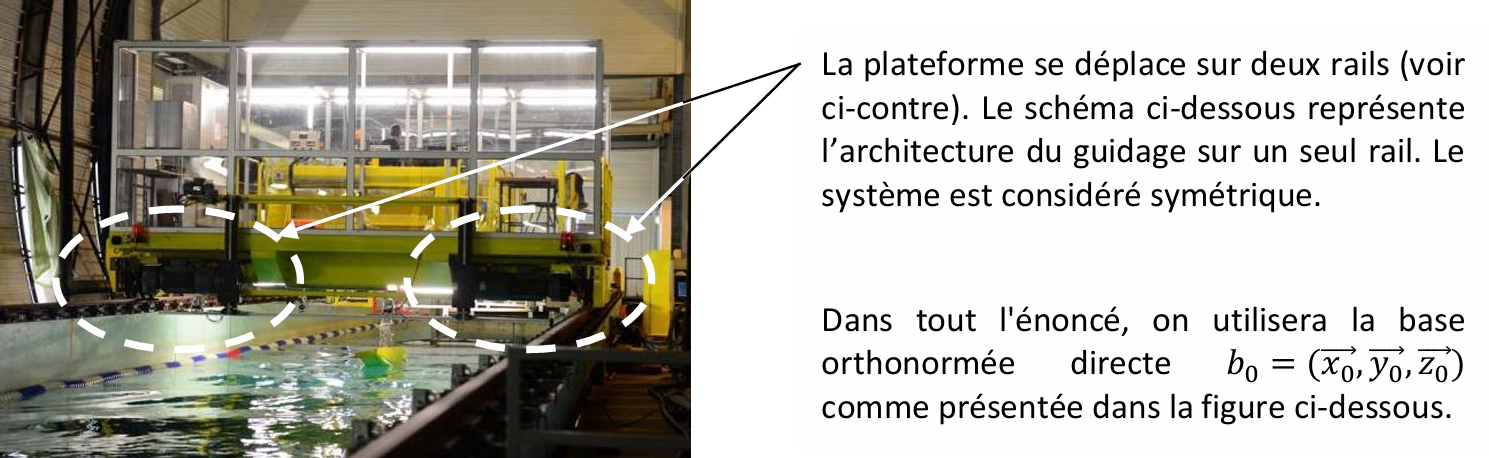
\includegraphics[width=\linewidth]{annexe6}
\end{center}

\begin{center}
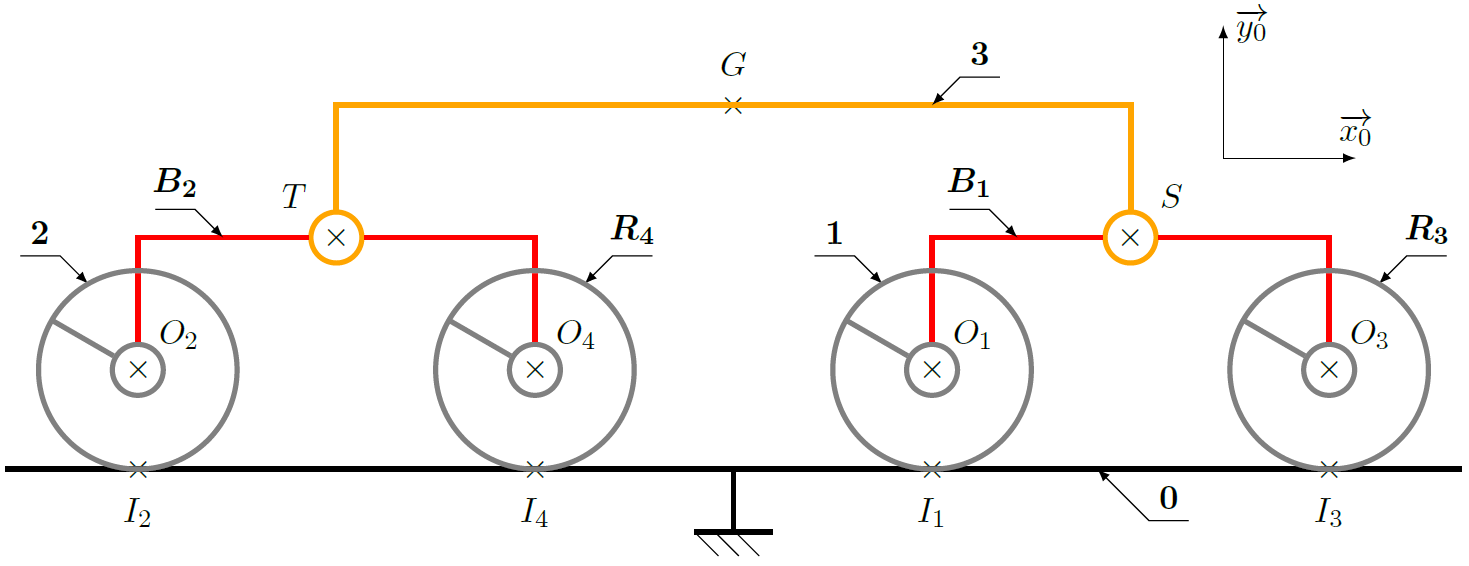
\includegraphics[width=\linewidth]{ann_08}

\textit{Schéma cinématique complet du chariot }
\end{center}
\subsection*{Annexe 7 -- Dispositif de mesure -- Photos et modèle retenu}

\begin{center}
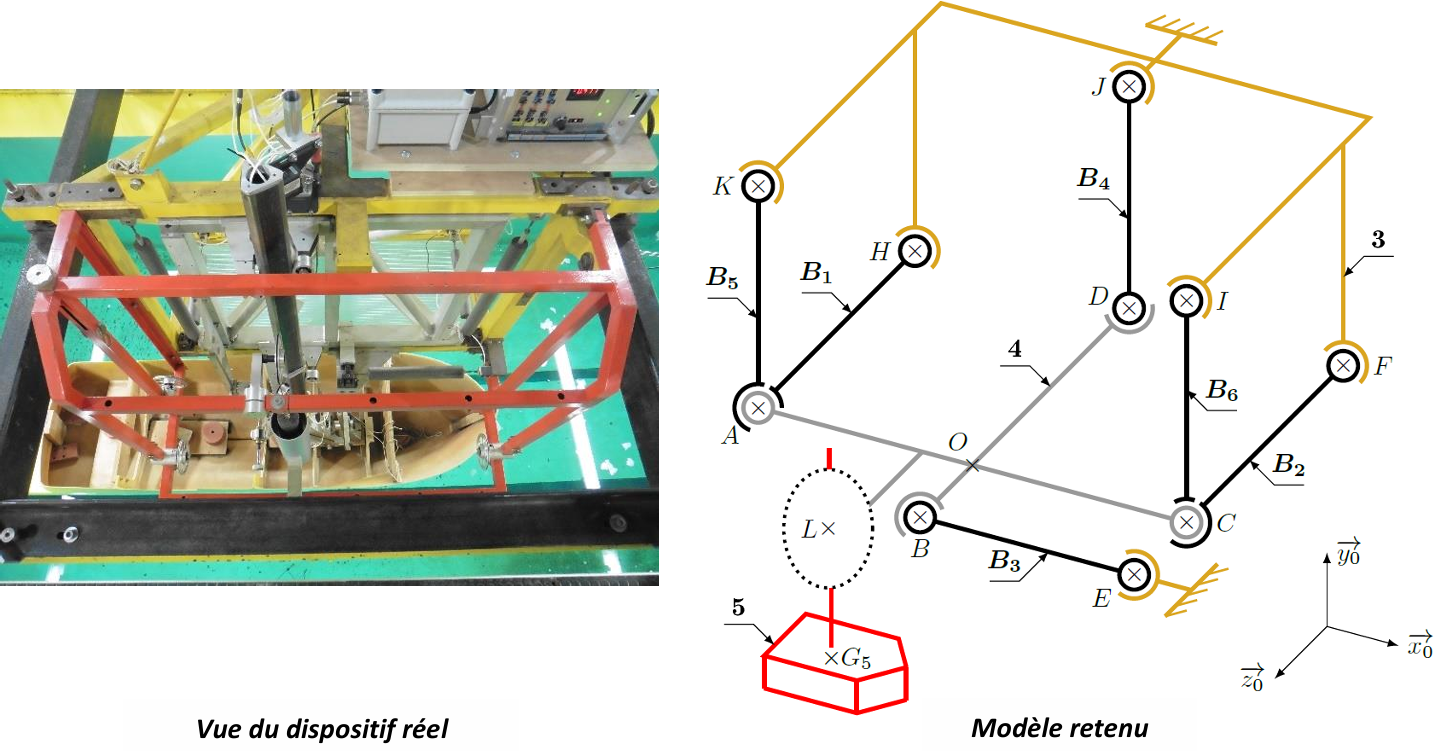
\includegraphics[width=\linewidth]{ann_07a}
\end{center}

\vspace{1cm}

\begin{center}
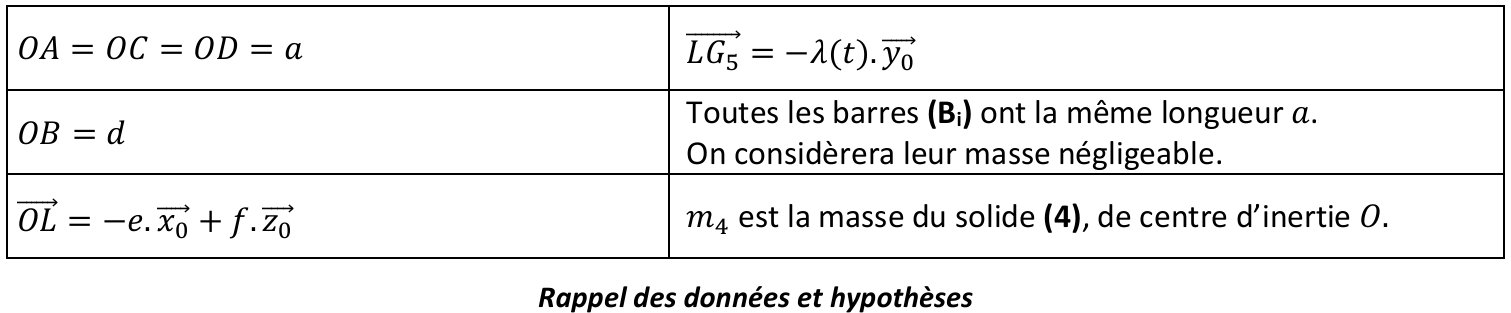
\includegraphics[width=\linewidth]{ann_07b}
\end{center}

\vspace{1cm}

\begin{center}
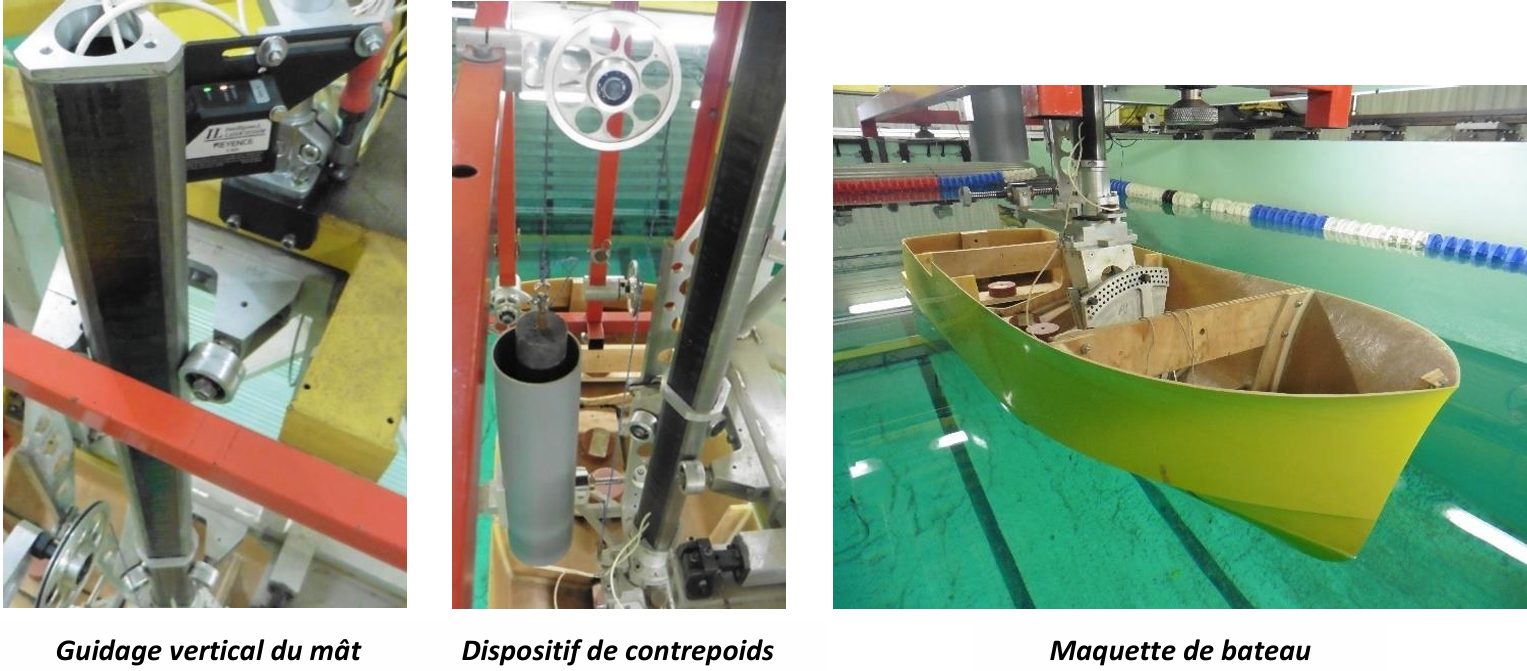
\includegraphics[width=\linewidth]{ann_07c}
\end{center}
